\documentclass{sig-alternate}
\usepackage{algorithmic}
\usepackage{algorithm}

\begin{document}
\conferenceinfo{GECCO'12,} {July 7-11, 2012, Philadelphia, Pennsylvania, USA.}
\CopyrightYear{2012}
\crdata{978-1-4503-1177-9/12/07}
\clubpenalty=10000
\widowpenalty = 10000
    
\title{Accelerating Evolution via Egalitarian Social Learning}

\numberofauthors{1}
\author{
\alignauthor
Wesley Tansey, Eliana Feasley, Risto Miikkulainen\\
       \affaddr{Dept. of Computer Science, The University of Texas at Austin}\\
       \affaddr{1 University Station C0500, Austin, TX, USA}\\
       \email{\{tansey, elie, risto\}@cs.utexas.edu}
}
\date{25 January 2012}

\maketitle
\begin{abstract}
Social learning is an extension to evolutionary algorithms that enables agents to learn from observations of others in the population. Historically, social learning algorithms have employed a student-teacher model where the behavior of one or more high-fitness agents is used to train a subset of the remaining agents in the population. This paper presents an egalitarian model of social learning in which agents are not labeled as teachers or students, instead allowing any individual receiving a sufficiently high reward to teach other agents to mimic its recent behavior. We validate our approach through a series of experiments in a robot foraging domain, including comparisons of reward-based social learning with simple neuroevolution and a variant of student-teacher social learning. The egalitarian algorithm converges to near-optimal strategies faster than either benchmark approach, outperforming both in a complex foraging task by more than an order of magnitude. The results indicate that egalitarian social learning is a promising new paradigm for social learning in intelligent agents.
\end{abstract}

\terms{Social Learning, Evolutionary Algorithms, Artificial Life, Cultural Algorithms, On-line Evolution}

\section{Introduction}

Evolutionary Algorithms (EAs) \cite{fogel1966artificial} evaluate agents either in isolation or in direct competition with a subset of the other members of the population. Social and cultural learning algorithms \cite{reynolds1994introduction} extend EAs by enabling agents to leverage observations of other members of the population to improve their own performance during their lifetime. By learning from others without having to directly experience or acquire knowledge, social learning algorithms have been able to improve the learning rate of EAs in many challenging domains \cite{denaro1996cultural, haasdijk2008social, vogt2010modeling, acerbi2007social, de2011incremental, watkins1992q}.

Traditionally in social learning algorithms, each agent is either a student or a teacher \cite{TODO}. All actions of the teacher agents are considered to be good examples from which to learn, as they are derived from a high-fitness strategy (i.e., the teacher's policy). However, an agent with high overall fitness may not always choose good actions and agents with low overall fitness may actually perform well in some limited scenarios. Filtering potential observations based on their own merit therefore may be more appropriate and lead to both improved learning rate and stronger final strategies.

In this paper, we present an Egalitarian Social Learning (ESL) as an alternative to the student-teacher paradigm. Agents in ESL are divided into subcultures at the start of each generation and can learn from any other agent in their subcultural group. The choice of learning examples is determined by a user-defined acceptability function that filters out examples leading to low rewards. When an acceptable action is observed, agents mimic that action in order to learn a policy similar to that of the observed agent. ESL differs from other social learning algorithms in that the quality of a training example is measured by the reward received rather than the fitness of the agent generating the example.

%inspired by mirror neurons \cite{gallese-98}, in which agents learn by observing the actions of other individuals. Primate brains contain mirror neurons that activate when other primates are observed, in effect mirroring the observed primate's action internally. Analogously, agents in our algorithm observe the population and, when a positive reward is received, mimic that action in order to learn a policy similar to that of the observed agent. This algorithm separates itself from other social learning algorithms in that the quality of a training example is measured by the reward received rather than the hierarchical role of the agent generating the example.

We validate our algorithm in a well-known foraging domain in which agents must learn to navigate the world efficiently, gathering nutritious food while avoiding poisonous food. The empirical results indicate that egalitarian social learning is able to quickly find near-optimal strategies more than an order of magnitude faster than a student-teacher variant and plain neuroevolution. Additionally, the use of subcultures in ESL is shown to promote behavioral diversity and prevent premature convergence to sub-optimal strategies that would otherwise emerge if agents observed all individuals in the population.

This paper makes the following contributions:
 
\begin{itemize}
\item An egalitarian social learning algorithm, in which all individuals in a subculture observe, learn from, and teach each other;
\item A behavioral diversity analysis of two egalitarian social learning variants;
\item A performance comparison between ESL and traditional student-teacher social learning.
\end{itemize}
 
The remainder of the paper is structured as follows.
Background information and prior work is discussed in Section \ref{sec:background}.
Section \ref{sec:rbsl} details the how the Egalitarian Social Learning algorithm works. Section \ref{sec:setup} describes both the experimental setup and the foraging domain in detail.
Section \ref{sec:results} presents experimental results.
A discussion of the results and planned future work are described in Section \ref{sec:future}.
Finally, in Section \ref{sec:conclusions} we present our conclusions.

\section{Background}
\label{sec:background}
In this section, background information and motivation for social learning is provided, as well as an introduction to the evolutionary framework underlying ESL.

\subsection*{Social Learning}

One explanation for the evolution of large brains in primates is the social intelligence hypothesis\cite{TODO}, which states that the need to handle complex social behaviors was the primary selection pressure driving the increase in brain size. The cultural intelligence hypothesis extends this concept solely to humans, stating that our brains evolved to handle the specific challenge of culture creation and social learning. These hypotheses are currently the most widely accepted explanations for the evolution of the human brain among evolutionary biologists and cognitive scientists \cite{holekamp2007questioning}, and have been supported by strong empirical evidence in recent years \cite{herrmann2007humans}.

Cultural and social learning algorithms \cite{reynolds1994introduction} model this biological mechanism in multi-agent systems by designating teacher agents that propagate knowledge and train other agents in the population. These techniques effectively enhance EAs with a hierarchical structure (i.e., students and teachers) that makes it possible to discover suitable actions to use as training examples and target individuals to train. Typical cultural algorithms therefore capture the ability of humans to learn from formal instruction by an expert, but they do not fully model all forms of learning from observation in primates. For instance, human brains contain mirror neurons \cite{gallese-98} that activate when other humans are observed interacting with the world, in effect mirroring the observed human's action internally. Such processes enable humans to learn socially without concern for the status or expertise of the observed individual.

\subsection*{Related Work}

Enhancing EAs with social learning is a flourishing area of research with a long and successful track record. This section highlights relevant prior work and explains how ESL differs from previous efforts.

Cultural algorithms \cite{reynolds1994introduction} have been used frequently in Particle Swarm Optimization (PSO) \cite{kennedy1995particle}. These algorithms maintain a ``belief space'' representing different categories of knowledge that the population has learned. New individuals are trained using this belief space in a student-teacher paradigm. In contrast, ESL agents maintain no separate repository of formal knowledge, but rather they learn from observations of others during their lifetime.

Interestingly, ESL could be seen as a Memetic Algorithm (MA) \cite{moscato1989evolution}. As originally defined by Dawkins \cite{dawkins2006selfish}, a meme is a ``unit of imitation in cultural transmission'' including ``tunes, ideas, catch-phrases, clothes fashions, ways of making pots or of building arches''. Knowledge propagation in ESL particularly relates to the latter--- ways of making pots or building arches are similar to strategies for gathering food in that they all are instances of transmitting specific strategies for performing skilled tasks. Thus, each acceptable learning example could be considered as a meme being shared within the agent's subculture. Nevertheless, traditional MAs \cite{onwubolu2004new}, including similar Lamarckian evolution methods for evolving recurrent neural networks \cite{ku2000study}, focus on using local improvement heuristics and typically rely on off-line transmission of memes via mating and genetic recombination. However, agents in ESL transmit memes on-line as they are generated and observed during the evaluation process. Thus, while we could classify ESL as an MA, we believe the distinct transmission and learning techniques employed by the algorithm better characterize it as a social learning method.

The ability of social learning to improve agents in a foraging domain has been explored by several researchers in recent years. Denaro et. al. \cite{denaro1996cultural} used a student-teacher model of cultural evolution without genetic inheritance and demonstrated that the population will continue to improve if Gaussian noise is added to the training examples. The NEW TIES system \cite{haasdijk2008social, vogt2010modeling} simulates a steady-state evolution of decision tree agents where at each step the teacher agents probabilistically transmit their decisions and students probabilistically incorporate this knowledge. Acerbi et. al. \cite{acerbi2007social} use social learning to train embodied agents to mimic the behaviors of more experienced agents. Finally, de Oca et. al. \cite{de2011incremental} propose a methodology for incremental social learning in PSO to update Q-learning \cite{watkins1992q} value functions by randomly selecting two individuals from the population and combining their values for a given update. While all of these studies are closely related and motivated by similar biological processes as ESL, they fundamentally all rely on the concept of students and teachers, and perform either no filtering or a reward-agnostic filtering of state-action pairs to be used in updating the population.

\subsection*{Evolutionary Framework}
NeuroEvolution of Augmenting Topologies (NEAT)\cite{stanley2002evolving} is an evolutionary algorithm that generates recurrent neural networks. Through a process of adding and removing nodes and changing weights, NEAT evolves genomes that unfold into networks. In every generation, those networks with the highest fitness reproduce, and with the lowest fitness are unlikely to do so. NEAT maintains genetic diversity through speciation and encourages innovation through explicit fitness sharing.

In the foraging domain, NEAT is used to generate a population of individual neural networks that control agents in the world. The input to each network is the agent's sensors, and the outputs control the agent's velocity and orientation. The fitness of each network is determined by the success of the agent it controls - over the course of a generation, networks that control agents who eat a good deal of rewarding food and very little poison will have high fitnesses and those that control agents with less wise dietary habits will have low fitness.

In standard NEAT, the networks that are created do not change within one generation. To facilitate social learning, we must perform backpropagation \cite{rumelhart1986learning} on the networks that NEAT creates in order to train agents on accepted examples. Since NEAT networks are recurrent, ESL enhances NEAT with backpropagation capabilities using the backpropagation through time \cite{werbos1990backpropagation} algorithm.

The final fitness of each phenome, then, reflects the performance of the individual that used that phenome and elaborated on it over the course of a generation. This elaboration drives evolution in two alternate ways.  In Darwinian evolution, the changes that were made to the phenome only affect selection and are not saved; in Lamarckian, the genome itself is modified.

\section{Egalitarian Social Learning}
\label{sec:rbsl}

Algorithm \ref{reward-algorithm} presents the on-line, generational learning algorithm for Egalitarian Social Learning. The algorithm is designed for domains where an agent receives multiple rewards throughout its lifetime. Agents maintain a sliding window of their most recent states, actions, and rewards that serve as training examples for observing agents. When an agent receives a reward, other agents observe the event and determine if it qualifies as an acceptable training example. The key insight in ESL is that the agents should focus on the event itself to determine if the observed actions should be emulated. The overall fitness of the acting agent is not considered, as it is possible that a low-fitness strategy may perform high-quality actions in certain circumstances.

To promote diversity and prevent the population from prematurely converging to local optima, all agents are divided into observation groups called \textit{subcultures}. At each timestep, each agent observes its state, responds with a desired action, and receives a resulting reward. The memory of an individual agent is thus a tuple containing its most recent state, action, and reward. Each agent's memory is evaluated by all other members of its subculture using a user-defined acceptability function. The role of this function is to filter out low-quality examples and focus the agents on learning only from actions that will lead to strong strategies. When an agent's recent memory is judged as acceptable, it is then used as a teaching example for all other agents in its subculture.

\begin{algorithm}
\caption{Egalitarian Social Learning}
\label{reward-algorithm}
\begin{algorithmic}
\STATE \textbf{Input:} $generations, maxTimesteps$
\STATE $population \leftarrow$InitializePopulation()
\STATE $g \leftarrow 0$
\STATE $t \leftarrow 0$
\LOOP
\WHILE{$g < generations$}
  \STATE $subcultures \leftarrow$ FormSubcultures($population$)
  \WHILE{$t < maxTimesteps$}
    \FOR{each $subculture$ in $subcultures$}
      \FOR{each $agent$ in $subculture$}
        \STATE $s \leftarrow $ReceiveAgentInputs()
        \STATE $a \leftarrow $GetResponse($agent, s$)
        \STATE $r \leftarrow $TakeAction(action)
        \STATE $agent.memory \leftarrow $UpdateMemory($\{s, a, r\}$)
      \ENDFOR
    \FOR{each $agent$ in $subculture$}
      \IF{Acceptable($agent.memory$)}
        \FORALL{$observer$ in $subculture$}
          \STATE Train($observer, agent.memory$)
        \ENDFOR
      \ENDIF
    \ENDFOR
    \ENDFOR
    \STATE $t \leftarrow t + 1$
  \ENDWHILE
  \STATE $population \leftarrow$SelectAndReproduce($population$)
  \STATE $g \leftarrow g + 1$
\ENDWHILE
\ENDLOOP
\end{algorithmic}
\end{algorithm}

% \begin{figure}
%   \centering
%     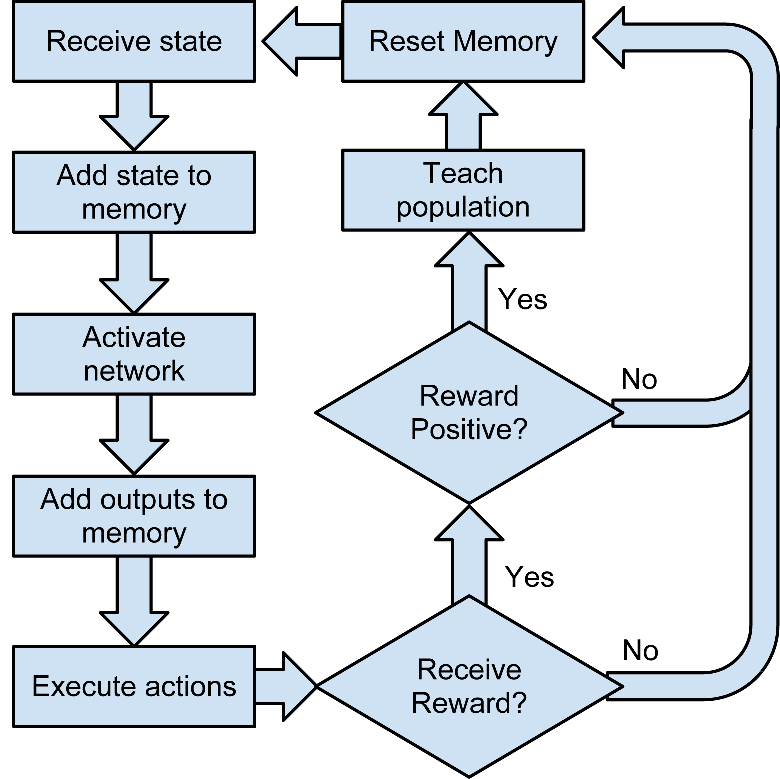
\includegraphics[scale=.6]{flowchart.pdf}
%   \caption{Individuals remember their most recent inputs and the associated actions taken, and when rewarded will train other individuals on their recent actions.}
%   \label{fig:flowchart}
% \end{figure}

%As a pragmatic note, by focusing on rewards rather than overall agent fitness, social learning can begin immediately in the first generation of the algorithm. In contrast, generational student-teacher models typically require a preliminary evaluation phase to determine high-quality agents and an off-line teaching phase to train new agents \cite{denaro1996cultural}. Thus, we expect our approach to be faster in practice as well as potentially producing stronger strategies.

The next section presents the experimental domain used to evaluate the efficacy of reward-based social learning.

\section{Experimental Setup}
\label{sec:setup}
This section describes the evaluation domain, including the inputs and outputs that agents receive, and the common parameters across all experiments.

\begin{figure}[t]
  \centering
    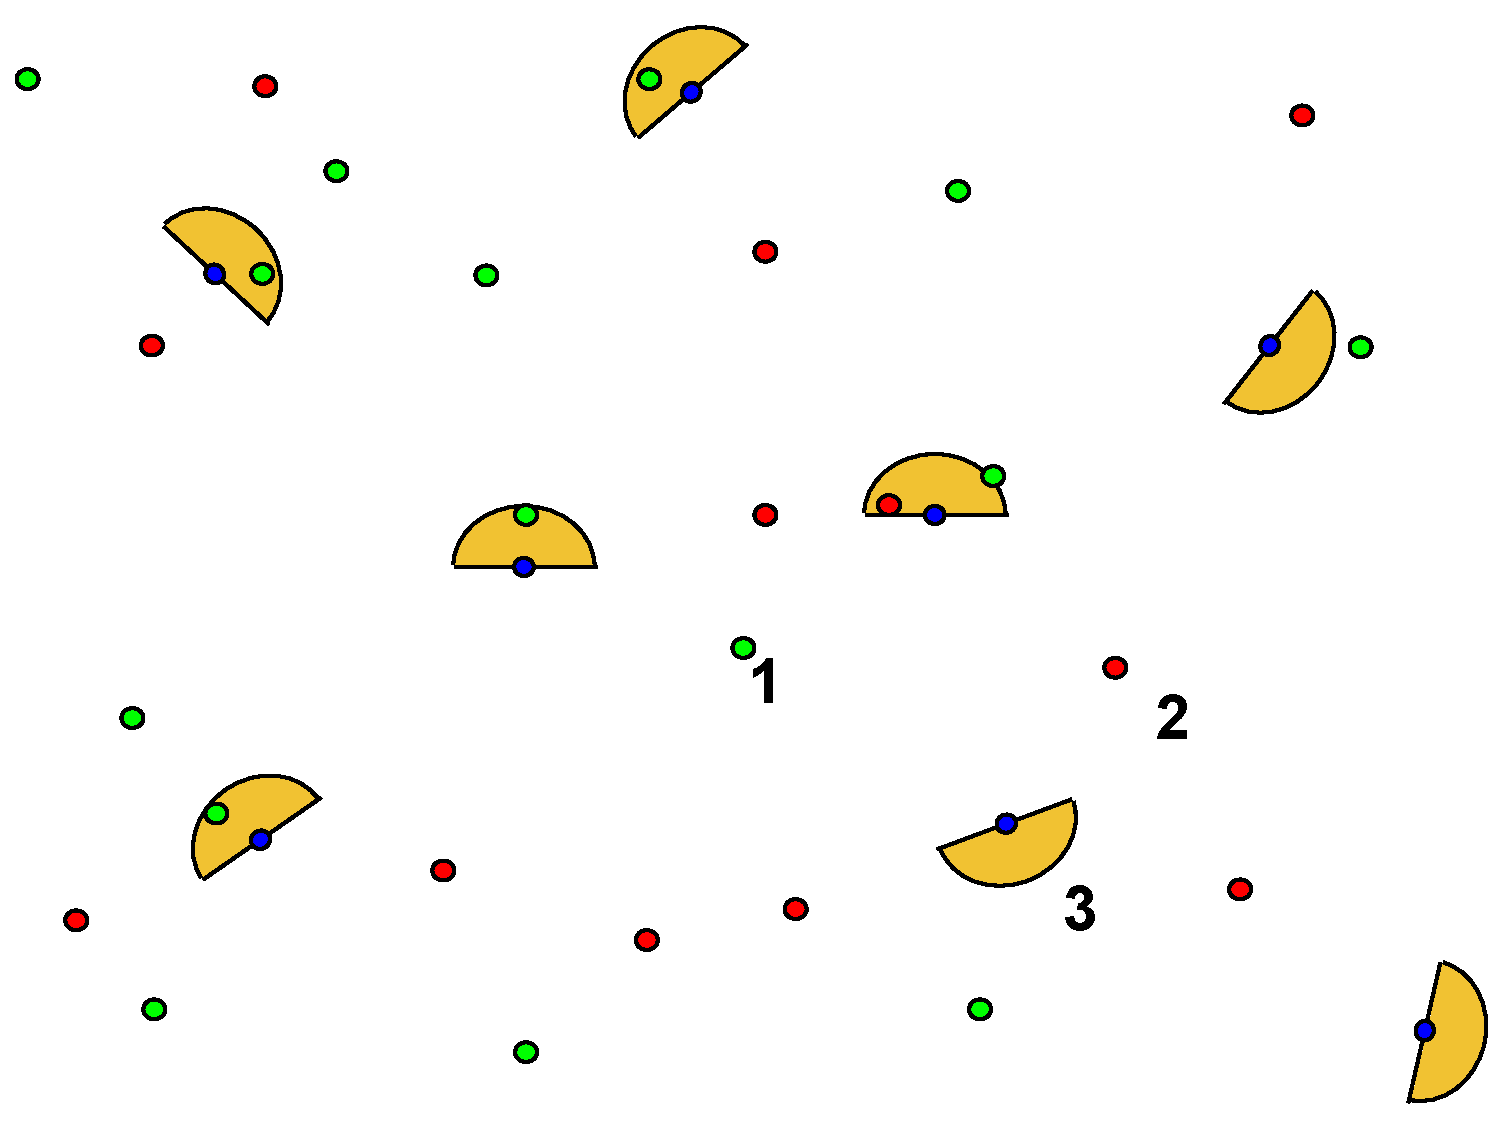
\includegraphics[scale=.31]{world.pdf}
  \caption{Our domain: a foraging world in which agents gain fitness by consuming plants which they approach.  1) a piece of nutritious food which increases fitness, 2) is poison which decreases fitness, and 3) is one of our agents.}
  \label{fig:foraging-world}
\end{figure}

\subsection*{The Foraging Domain}
The domain used to evaluate ESL is a foraging world in which agents move freely on a continuous toroidal surface. The world is populated with various plants, some of which are nutritious and bear positive reward, while others are poisonous and bear negative reward. These plants are randomly distributed over the surface of the world. The foraging domain is non-competitive and non-cooperative; each agent acts independently of all other agents, with the exception of the teaching signals that pass between them. At the start of each generation, all individuals begin at the center of the world, oriented in the same direction, and confronted with the same plant layout and configuration. Every agent then has a fixed number time steps to move about the surface of the world eating plants--- which happens automatically when an agent draws sufficiently close to one--- before the evaluation is over. Figure \ref{fig:foraging-world} shows an example of a foraging world with two types of plants and eight agents.
    
\begin{figure}[t]
  \centering
    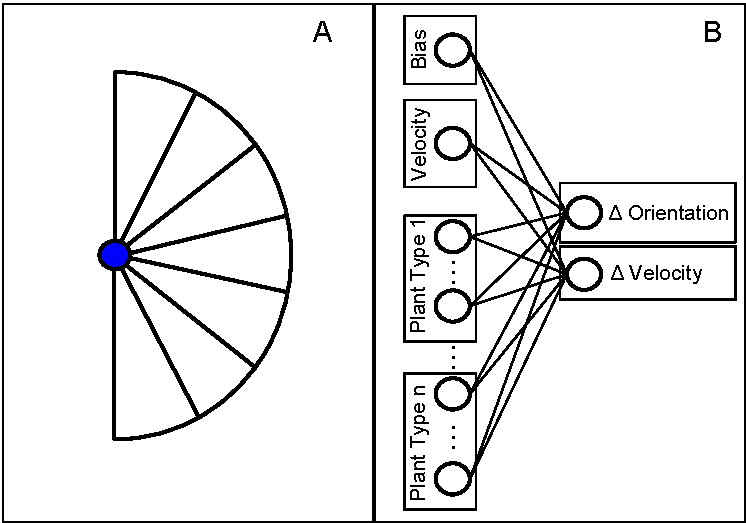
\includegraphics[scale=.665]{foraging_agent_architecture.pdf}
  \caption{The architecture of foraging agents. A) Each agent has a 180$^{\circ}$ field of vision, discretized into eight sensors for each plant type. B) Each agent is controlled by a neural network taking the agent's current velocity and sensor activations as inputs and outputting the desired change in orientation and velocity.}
  \label{fig:agent-architecture}
\end{figure}

\subsection*{Sensors and Outputs}

Agents ``see'' plants within a 180$^\circ$ horizon via a collection discretized sensors. Each agent has eight sensors for each type of plant, with each sensor covering a different 12.5$^\circ$ sector of the 180$^\circ$ ahead of the agent. Agents cannot see other individuals or plants they have already eaten--- all they can see is edible food. The strength of the signal generated by each plant is proportional to its proximity to the agent. Agents also have a sensor by which they can detect their current velocity. As agents can only turn up to 30$^\circ$ in a given timestep, knowledge of velocity is necessary for agents to accurately plan optimal trajectories (e.g., if it needs to slow down in order to prevent overshooting a plant).  Each agent is controlled by an artificial neural network that maps from the agent's sensor readings to the desired change in orientation and velocity. Figure \ref{fig:agent-architecture} shows the architecture of a foraging agent.

\subsection*{Common Parameters}

Two separate configurations of the robot foraging world are used in the experiments. The first three experiments use a ``simple'' world where the toroidal surface is 2000 by 2000 units, with a single plant type of value 100 and 50 randomly distributed instances of the plants. In this world, the agents have a straight-forward task of learning to navigate efficiently and gather as many plants as possible.

The fourth set of experiments uses both the simple world and a second, more complex world to evaluate performance. The ``complex'' world has a surface of 500 by 500 units, with five different plant types of value -100, -50, 0, 50, and 100. For each plant type, 20 plant instances are created and randomly distributed across the surface. This world presents the agents with a more difficult task as they must both efficiently gather nutrious food while simultaneously avoiding the poisonous food.

In all four experiments, 100 different agents are created in each generation. All networks are initialized with fully-connected weights with no hidden neurons and a learning rate of 0.1 is used when performing backpropagation. Agents automatically eat any plant with which they are within five units. Each evaluation lasts 1000 timesteps and the results for each experiment are the average of 30 independent runs. The acceptability function for all experiments is to learn from any action yielding a positive reward.

The next section describes each experiment and its outcome in detail.

%In both worlds, there are 100 agents and when they are divided into cultural cliques, there are ten cliques of ten agents. Each agent had 8 different sensors for each type of plant, and automatically ate any plant it came within 5 units of. 

\section{Results}
\label{sec:results}
Four main experiments were conducted: 1) determining the baseline performance of egalitarian social learning and simple neuroevolution, each in isolation, 2) measuring the performance of a monocultural ESL in Darwinian and Lamarckian evolutionary paradigms, 3) evaluating whether subcultural learning improves performance compared to having a monoculture population, and 4) comparing ESL to a student-teacher learning algorithm in both simple and complex foraging tasks. The first three experiments examine the efficacy of the various components of the ESL algorithm while the fourth experiment serves to validate the final algorithm against a variant of a related approach in the literature. The experimental results show that ESL is able to evolve high-quality strategies with substantially fewer agent evaluations than previous algorithms.

%determining the feasibility of reward-based social learning in isolation without any evolution and establishing a baseline result for pure neuroevolution with no on-line learning

\begin{figure}
  \centering
    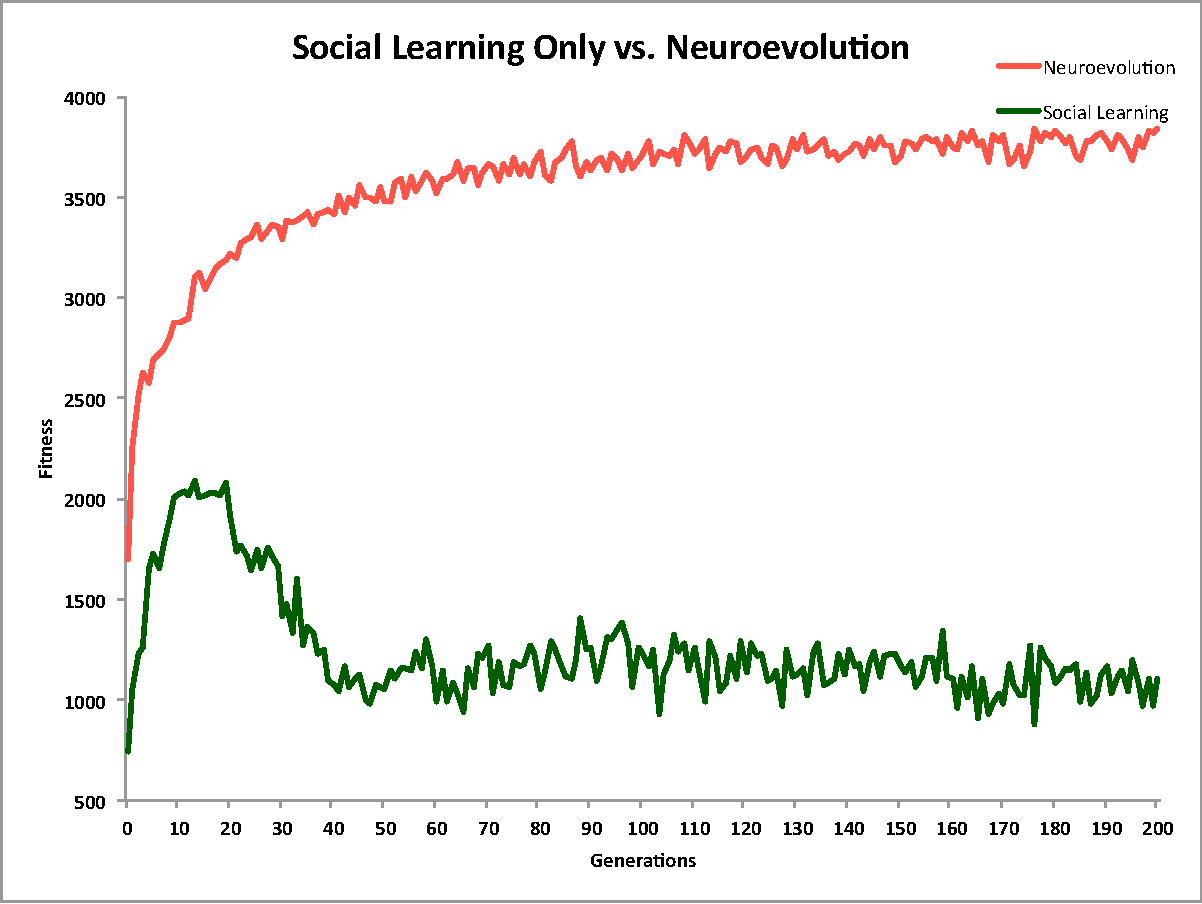
\includegraphics[scale=.41]{social_learning_vs_neuroevolution.pdf}
  \caption{Pure reward-based learning collapses after several generations, while neuroevolution alone converges to a stable but suboptimal solution.}
  \label{fig:social-neuro}
\end{figure}

\subsection*{Egalitarian Learning vs. Neuroevolution}

The first experiment establishes a baseline for understanding the ability of our two component methods, social learning and neuroevolution, to evolve high-quality strategies in isolation. To evaluate social learning in isolation, a monocultural population of 100 randomly initialized neural networks is created and evaluated without selection or reproduction for 200K time steps. After every 1000 time steps, the population champion is recorded and this is treated as a ``generation'' in order to compare it to simple neuroevolution.

Figure \ref{fig:social-neuro} shows the results of the experiment. While egalitarian social learning alone is able to improve initially, after several epochs a regression-to-the-mean effect is observed in which the entire population converges to a mediocre average score. A similar effect has been observed in previous social learning experiments \cite{denaro1996cultural}, suggesting that some form of mutation is needed to prevent population collapse. In contrast, neuroevolution converges to solutions with fitnesses two to three times higher than that of reward-based social learning alone after approximately 50 generations.

Having validated that social learning alone is not sufficient, the next experiment compares the performance of social learning when used as an enhancement to two different forms of simulated evolution.

\subsection*{Darwinian vs. Lamarckian Evolution}

Genetic inheritance paradigms in evolution fall into one of two main categories: Darwinian and Lamarckian. In Darwinian evolution, individual genomes are fixed and any knowledge or abilities gained during their lifetimes are not passed on to their offspring at birth. By contrast, in Lamarckian evolution an individual's genome changes as it learns throughout its life, and these changes are passed on to each of its offspring. In the context of neuroevolution, this corresponds to whether the changes in each individual's neural network weights, as a result of social learning, are propagated to their genome at the end of the generation.

\begin{figure}
  \centering
    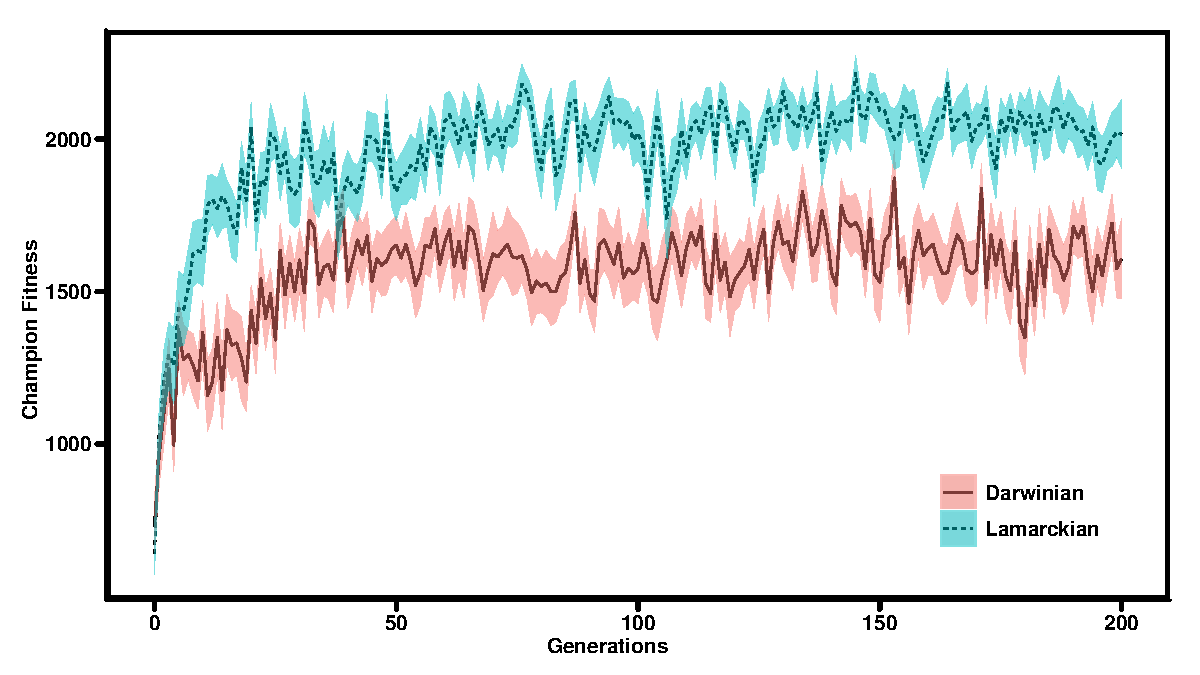
\includegraphics[scale=.41]{darwinian_vs_lamarckian_evolution.pdf}
  \caption{Lamarckian learning is more effective than Darwinian and converges more rapidly.}
  \label{fig:darwin-lamarck}
\end{figure}


Figure \ref{fig:darwin-lamarck} shows the results of applying a monocultural egalitarian social learning algorithm to the foraging domain in both the Lamarckian and Darwinian paradigms. The performance of both algorithms quickly converges, with Lamarckian reaching a higher-fitness solution than Darwinian evolution. In the context of \textit{on-line} evolutionary learning algorithms, previous work \cite{whiteson2006evolutionary} showed that Darwinian evolution is likely to be preferable to Lamarckian evolution in dynamic environments where adaptation is essential and the Baldwin effect \cite{simpson1953baldwin} may be advantageous. However, as adaptation is not necessary for foraging agents (i.e., the rewards of each plant type are the same in every generation), in this experiment Lamarckian evolution outperforms Darwinian evolution.

Nevertheless, in both cases performance converges to a lower score than that of simple neuroevolution. The next experiment presents the results of introducing subcultures into the egalitarian model to overcome such convergence tendencies.

\subsection*{Monocultural vs. Subcultural Learning}
On one hand, Lamarckian social learning is able to find good results quickly, while on the other hand, it is likely to provide redundant information that may result in getting stuck in local optima.  

In order to address this problem, we introduce a subcultural version of egalitarian social learning designed to promote and protect diversity. At the start of each generation, the population is divided into 10 subcultures of 10 agents each, with each agent's subculture decided at random. During the evaluation, agents only teach and learn from other agents in their own subculture. In addition to increasing behavioral diversity relative to learning from the entire population, this variant also has the appealing practical advantage that it decreases the worst-case number of iterations of backprop. For instance, in a population of 100 individuals with ten subcultures, an accepted training example is propagated to only 9 other agents, compared to 99 agents for the same example in a monocultural algorithm.

\begin{figure}
  \centering
    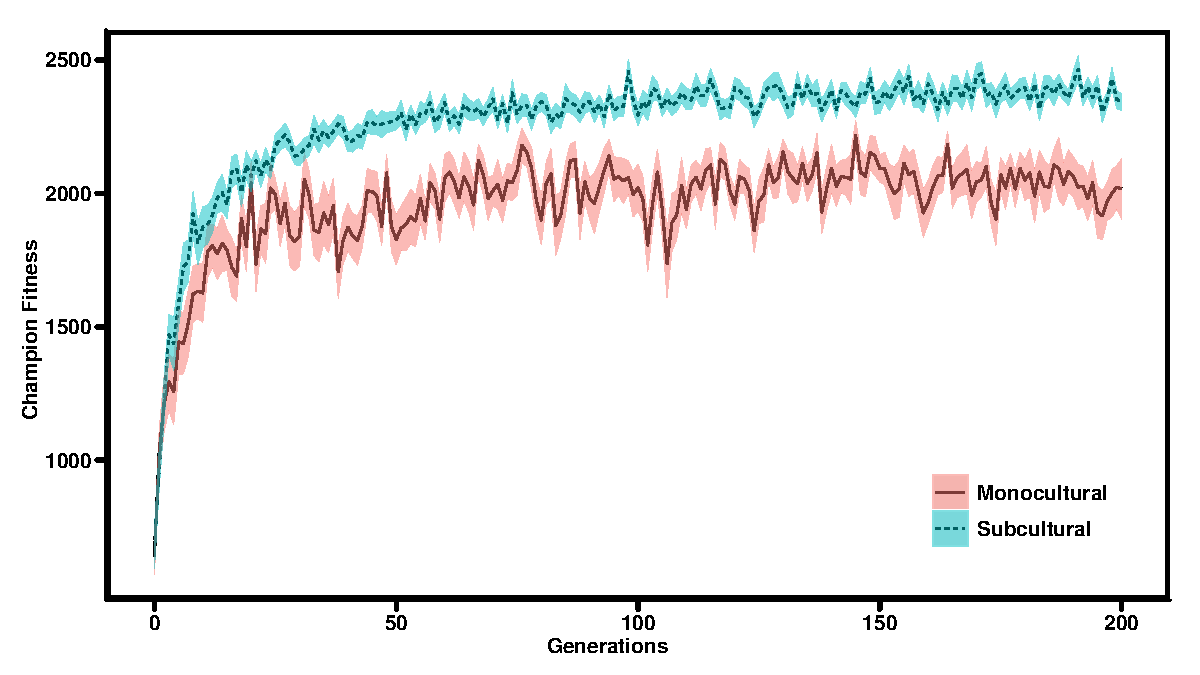
\includegraphics[scale=.41]{monocultural_vs_subcultural_learning.pdf}
  \caption{The results of agents learning from observations of the entire population compared to only agents in the same clique.}
  \label{fig:population-social}
\end{figure}

Figure \ref{fig:population-social} shows the results comparing population-based and cultural learning. The cultural social learning not only reaches a higher peak than the population-based method, but also arrives at this level of fitness more rapidly than the simple neuroevolution approach. Preventing agents that lead the population towards local optima from impacting the remainder of the population provides safety and protection from premature convergence; when every mutated organism has the opportunity to train every other, as is the case in monocultural learning, the entire population may be negatively impacted by such individuals. Because cultural evolution is more efficient and provides better results we incorporate it in our final algorithm.

\begin{figure}
  \centering
    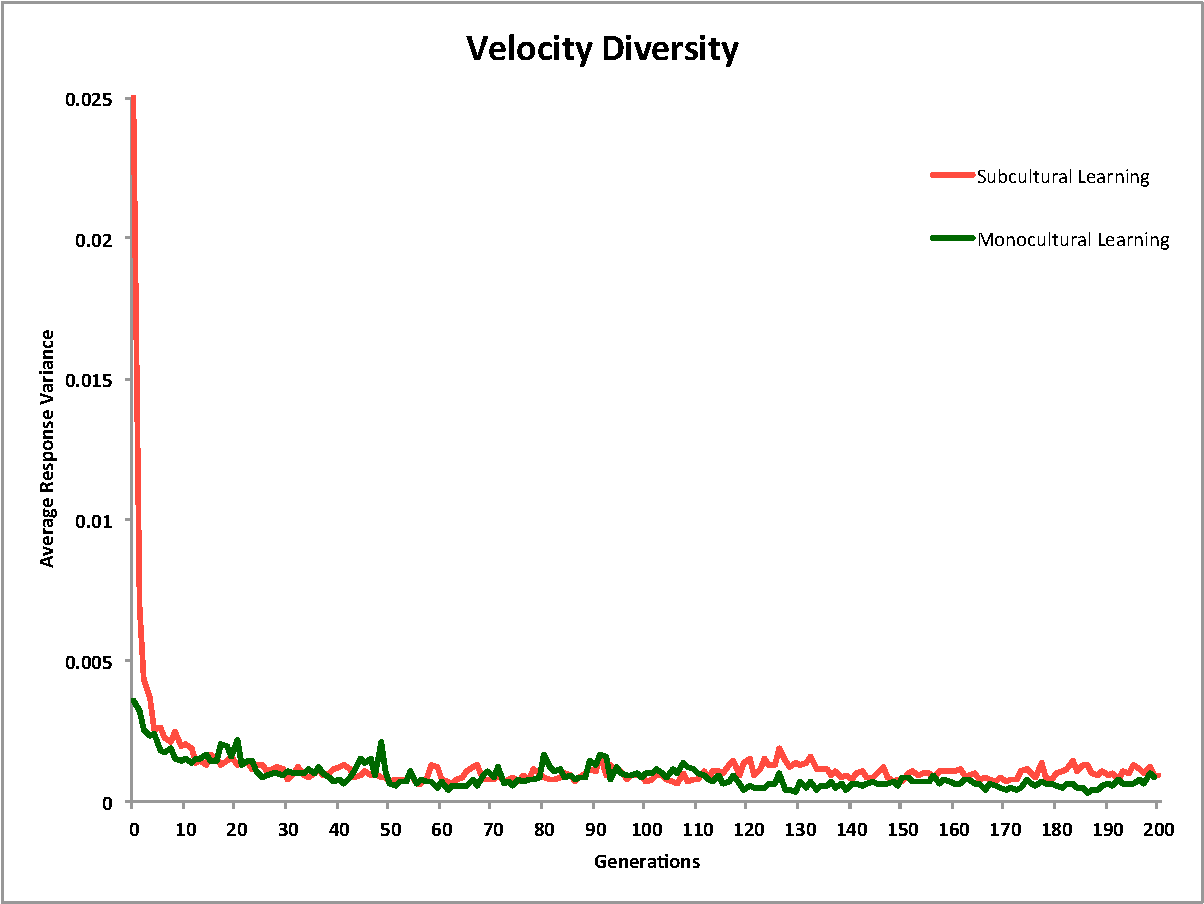
\includegraphics[scale=.41]{velocity_diversity.pdf}
  \caption{Velocity converges more quickly in the cultural model than in the population model.}
  \label{fig:velocity}
\end{figure}

\begin{figure}
  \centering
    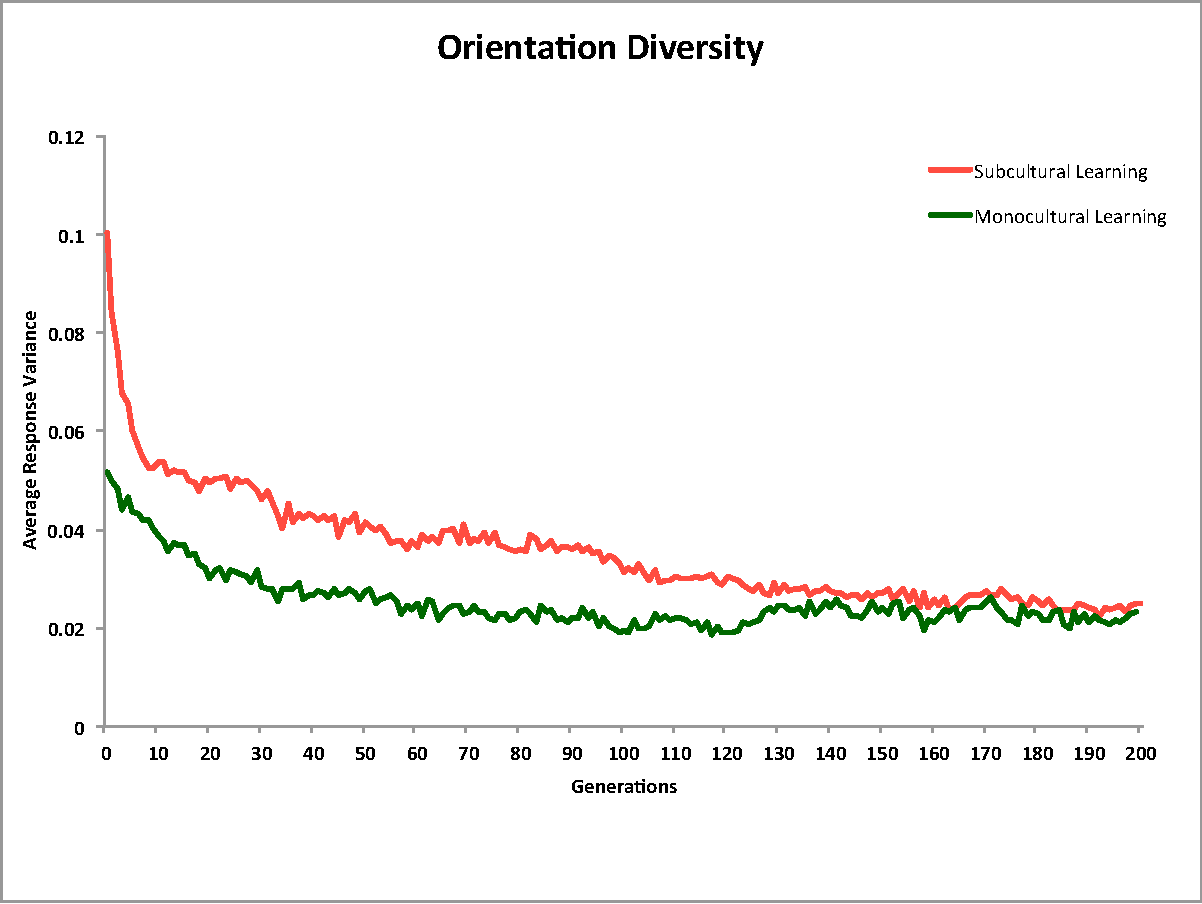
\includegraphics[scale=.41]{orientation_diversity.pdf}
  \caption{In the cultural learning model, diversity in terms of orientation is maintained for longer than in population learning before behavior converges.}
  \label{fig:orientation}
\end{figure}

To better understand why the cultural version of our algorithm was able to prevent premature convergence, the behavioral diversity of the population was analyzed after every generation. After each evaluation, a new instance of the simple world was generated and a set of input states was created corresponding to random locations, orientations, and velocities. For every agent, its output response (i.e., the desired change in velocity and orientation) was observed for each of the input states. Figures \ref{fig:orientation} and \ref{fig:velocity} show the average variance of the population response to each of the 100 input states after every generation, effectively measuring the behavioral diversity of the population.  Velocity response converges for both models almost immediately, while orientation response remains more diverse in subcultural than in monocultural learning.

Although the orientation and velocity results may seem contradictory, they actually reflect a desirable property of subcultural learning. In the case of velocity, both the population and cultural algorithms quickly converge to low diversity. Since even at full speed the agents can sense plants up to ten timesteps away, there is no clear benefit to slowing down in the current domain and one would expect a strong strategy to always output the maximum value for velocity. Thus, preserving diversity in this area would be detrimental to the performance of the population. Conversely, the diversity of orientation should be preserved, as there is a tradeoff between turning toward an immediate but small reward, such as a single plant within one step, and turning toward a delayed reward, such as a cluster of plants a few steps away. This complexity suggests that the fitness landscape for orientation  is likely filled with numerous local optima and diversity preservation should be beneficial to evolution. 

Thus the results of the diversity analysis suggest that the subcultural algorithm preserves diversity only when it is useful (e.g., orientation response), while not preventing convergence when diversity is unnecessary (e.g., velocity response).

The next experiment compares the ESL algorithm to a benchmark student-teacher model and plain neuroevolution.

\begin{figure}
  \centering
    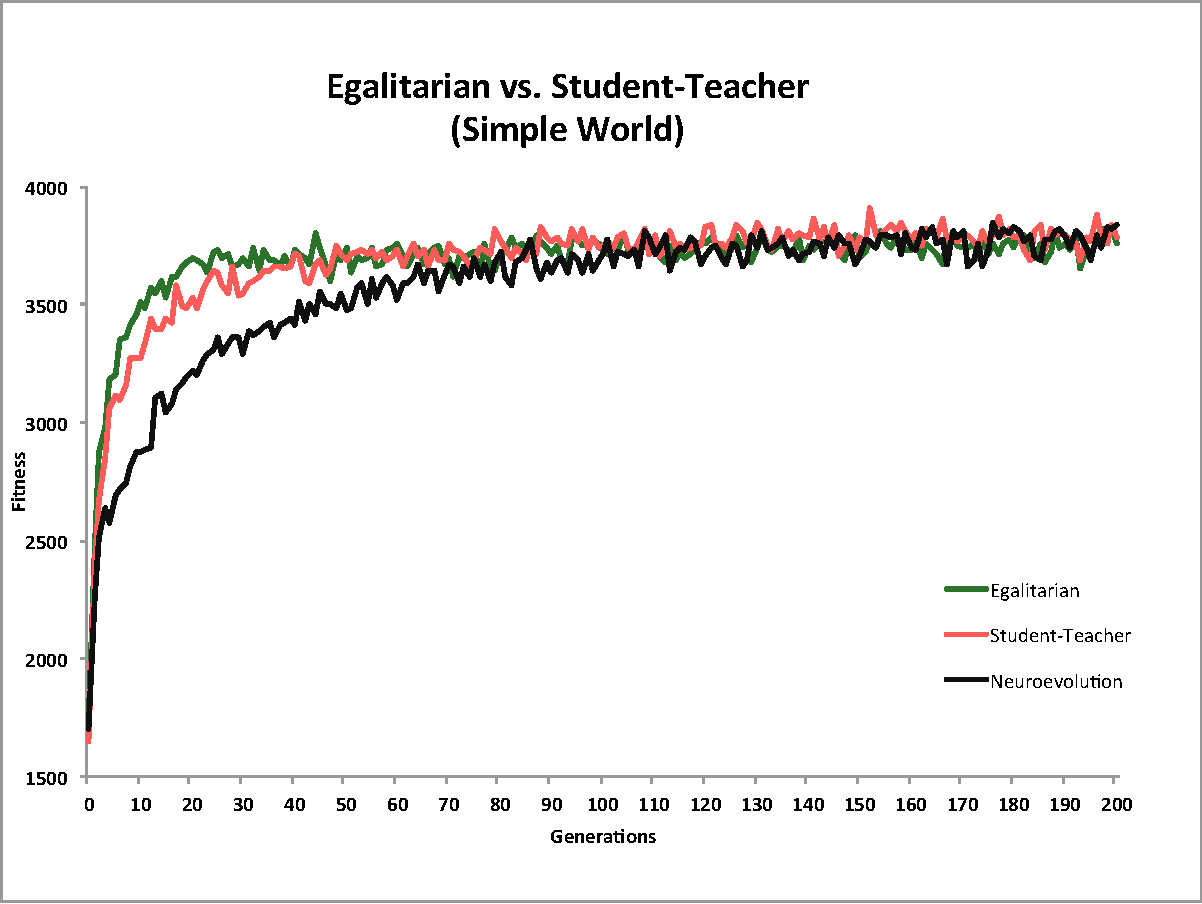
\includegraphics[scale=.41]{egalitarian_vs_student_teacher_simple.pdf}
  \caption{The results of our algorithm in a simple world evaluated alongside a more traditional student-teacher model and baseline pure neuroevolution.}
  \label{fig:reward-studentteacher-simple}
\end{figure}
\begin{figure}
  \centering
    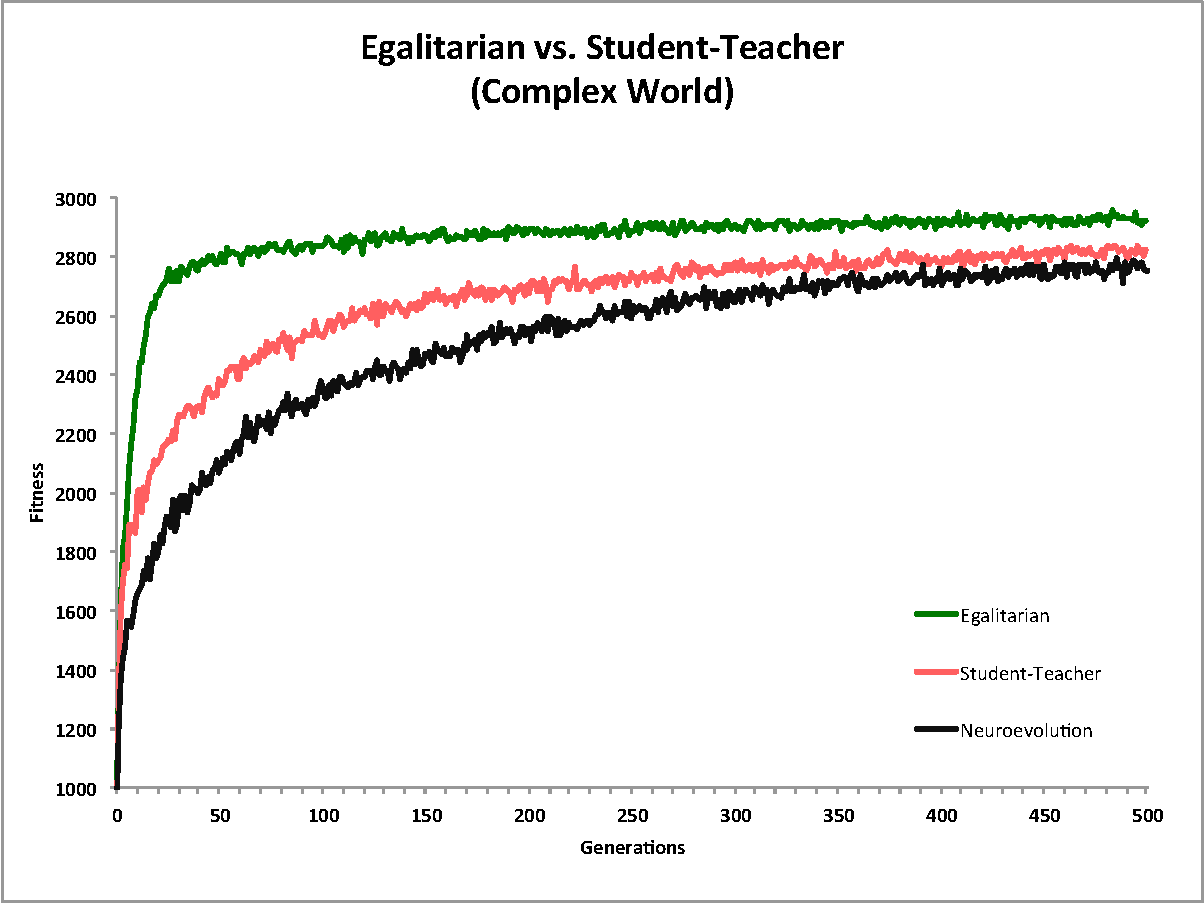
\includegraphics[scale=.41]{egalitarian_vs_student_teacher_complex.pdf}
  \caption{The results of our algorithm in a complex world evaluated alongside a more traditional student-teacher model and baseline pure neuroevolution.}
  \label{fig:reward-studentteacher-complex}
\end{figure}

\subsection*{Reward-Based vs. Student-Teacher}
In the final set of experiments, we compare our subcultural egalitarian algorithm to an on-line student-teacher learning algorithm inspired by the NEW TIES system \cite{haasdijk2008social}. The system utilizes a steady-state evolution in which at every timestep each agent probabilistically teaches the lowest-fitness member of the population within some radius, effectively forming geographical subcultures. The original system relies on a steady-state evolution where weaker agents eventually die out and do not have as much of a chance to propagate poor training examples as long-lasting agents. To adapt this approach to a generational EA, and to maximize the fairness of the comparison, a population of 10 subcultures is created with 10 agents each. At each time step, the current champion from each subculture teaches its group's lowest-fitness member on its most recent action regardless of whether the teaching agent received any reward.

It is worth noting that many social learning algorithms focus on off-line training, where teachers are simply the previous generation's champions. In these models, students are trained before the actual evaluation to mimic the champion(s), often with Gaussian noise added to the teacher's outputs to promote diversity in the population \cite{denaro1996cultural}. While such approaches may have also performed well in the foraging domain, they are not on-line learning algorithms. Rather, agents in these algorithms are static at evaluation time and do not learn from their own experiences or that of others. Thus, we chose to adapt the NEW TIES model to a generational EA as it is the most closely related approach in the literature.

Figures \ref{fig:reward-studentteacher-simple} and \ref{fig:reward-studentteacher-complex} show the results of the subcultural ESL algorithm compared to the student-teacher variant of NEW TIES and simple neuroevolution. Subcultural egalitarian learning converges to a near-optimal solution faster than the student-teacher variant in both the simple and the complex world. While in the simple world (Figure \ref{fig:reward-studentteacher-simple}) this speed-up is slight, in the complex world (Figure  \ref{fig:reward-studentteacher-complex}) the egalitarian approach is more than an order of magnitude faster, reaching a higher fitness by generation 50 than either the student-teacher or simple neuroevolution methods achieve by generation 500.

The next section presents a discussion of the experimental results and indicates possible future directions for ESL.

\section{Discussion and Future Work}
\label{sec:future}
The results of the above experiments in egalitarian social learning suggest that learning from strong actions, rather than high-fitness agents, is a powerful approach to social learning. The success of our algorithm in a given domain is predicated on two main user-defined parameters: the grouping of agents into subcultures and the criteria of the acceptability function.

For the experiments where subcultures were used, a simple division of 10 groups of equal size was chosen for the subculture creation strategy. Preliminary experiments showed that ESL results in the foraging domain were robust to moderate variations in the number of equal-sized subcultures, with 5 groups and 20 groups both demonstrating strong speedup compared to our benchmarks. However, it is possible that equal-sized groups are not optimal or that a dynamic subculture creation algorithm that maximizes behavioral diversity would perform better; such issues will be addressed in future work.

Creating an acceptability function is a closely related task to that of creating a fitness function. Consequently, the performance of ESL depends on the ability of the user to craft a useful acceptability function. This task is not always easy and may require paying attention to the subtle details of one's domain. The acceptability function was intentionally kept simple in both foraging domains so as to demonstrate the strength of the general egalitarian learning approach, however it is possible that employing a more sophisticated heuristic could speed up learning even more.

The robot foraging domain is well-suited for exploring extensions and improvements to egalitarian social learning. Whereas the current version only utilizes a single example at every time step, teaching more complex behaviors using reward-based approaches may require larger memory sizes. One interesting future work direction may be to introduce obstacles or walls that block the agent from immediately receiving the reward, necessitating that agents learn compound trajectories to navigate to the food.
%Additionally, we plan to introduce predators into the world and measure the effects reward-based social learning has when present in predators, prey, or both.

Finally, we plan to expand our benchmark suite to include more student-teacher variants in the future. Student-teacher methods can be implemented in many ways, including off-line learning \cite{acerbi2007social}, probabilistic teaching \cite{haasdijk2008social}, and noisy examples \cite{denaro1996cultural}, to name only a few. A more complete set of benchmarks will help us better understand the relative performance of each approach and how they compare to ESL both in the foraging domain and on future tasks.

%Future work may involve investigating the relationship between this and other forms of social learning and Q-learning.  Additionally, one strength of non-hierarchical social learning is its ability to transmit information about novel situations to all agents without those agents having to experience those situations themselves.  As such, investigating the impact of non-hierarchical social learning in dynamic domains with changing rewards is a promising and practical avenue for new research.  Finally, our current model teaches agents about the previous timestep with one iteration of backprop whenever there is a reward.  Extending the model to account for the magnitude of the reward, and to store and train on information about previous timesteps may lead to new insights.   

\section{Conclusions}
\label{sec:conclusions}

This paper presented an egalitarian approach to social learning in evolutionary algorithms that enables agents to learn from high-quality actions. As opposed to traditional social learning algorithms that follow a student-teacher model, our approach instead teaches agents based on acceptable actions taken by any agent in its subculture. By constraining teaching samples to those from the same subcultural group, our algorithm promotes diversity in the overall population and prevents premature convergence. Experiments in a complex robot foraging domain demonstrated that this approach is highly effective at quickly learning a near-optimal policy with Lamarckian evolution. Our results suggest that egalitarian social learning is a strong technique and represents a promising new paradigm for social learning algorithms.

\bibliographystyle{abbrv}
\bibliography{sigproc}


\end{document}